\documentclass[a4paper, 11pt]{quantumarticle}
\pdfoutput=1

\usepackage{amsmath, amssymb, amsthm}
\usepackage{graphicx}
\usepackage{booktabs}
\usepackage{hyperref}
\usepackage{cleveref}
\usepackage{algorithm}
\usepackage{algpseudocode}
\usepackage{tikz}
\usepackage{braket}
\usepackage{multirow}
\usepackage{xcolor}
\graphicspath{{figures/diagrams/}{figures/benchmarks/}}

% Theorem environments
\newtheorem{definition}{Definition}
\newtheorem{proposition}{Proposition}

% Shortcuts
\newcommand{\CC}{\mathbb{C}}
\newcommand{\RR}{\mathbb{R}}
\newcommand{\TT}{\mathcal{T}}
\newcommand{\LL}{\mathcal{L}}
\newcommand{\MM}{\mathcal{M}}
\newcommand{\II}{\mathbb{I}}
\newcommand{\tr}{\operatorname{tr}}
\newcommand{\diag}{\operatorname{diag}}
\renewcommand{\skew}{\operatorname{skew}}
\newcommand{\topk}{\operatorname{topk}}
\newcommand{\grad}{\operatorname{grad}}
\newcommand{\proj}{\operatorname{proj}}

\begin{document}

\title{Parametric Quantum Circuit Bases for Image Compression via Riemannian Optimization on Unitary Manifolds}

\author{Shiwen An}
\affiliation{Institute of Science Tokyo, Tokyo, Japan}
\author{Zhongyi Ni}
\affiliation{Hong Kong University of Science and Technology (Guangzhou), Guangzhou, China}
\author{Jin-Guo Liu}
\affiliation{Hong Kong University of Science and Technology (Guangzhou), Guangzhou, China}
\email{jinguoliu@hkust-gz.edu.cn}
\date{2026-03-18}

\maketitle

% ============================================================================
% ABSTRACT
% ============================================================================
\begin{abstract}
Compressed sensing relies on finding sparse representations of signals in a suitable transform basis.
Classical bases such as the Fourier and cosine transforms are fixed and signal-agnostic, leaving data-dependent structure unexploited.
We present a framework for learning data-adaptive unitary transforms by parameterizing the transform as a tensor network of quantum circuit gates and optimizing on the Riemannian manifold of unitary matrices.
The tensor network structure---inherited from the Cooley--Tukey decomposition of the FFT---provides an efficient $O(N \log N)$ transform while exposing a natural parameter manifold on which gradient-based optimization preserves unitarity exactly.
By varying the circuit connectivity, we construct a family of parametric bases with different inductive biases and systematically evaluate their compression quality.
We find that circuit topology is a more important design variable than parameter count: cross-dimensional entanglement gates that couple spatial dimensions yield the best performance, while topologies with only local connectivity underperform even the fixed FFT.
The approach combines tensor network contraction, Riemannian optimization, and differentiable programming, and is implemented as an open-source Julia library.
\end{abstract}

% ============================================================================
% INTRODUCTION
% ============================================================================
\section{Introduction}
\label{sec:introduction}

Sparse representation of signals is fundamental to data compression.
Classical transforms such as the Discrete Fourier Transform (DFT)~\cite{cooley1965fft} and the Discrete Cosine Transform (DCT)~\cite{ahmed1974dct} provide fixed bases with well-understood sparsity properties.
However, these bases are not adaptive to the statistics of specific signal classes.
In particular, the separable 2D DFT $F_m \otimes F_n$ treats spatial dimensions independently, ignoring cross-dimensional correlations common in natural images.

The Cooley--Tukey FFT algorithm admits a natural decomposition as a tensor network of two-qubit gates: Hadamard gates $H$ and controlled-phase gates $M_k = \diag(1, 1, 1, e^{i\pi/2^{k-1}})$.
With fixed parameters, this tensor network computes the DFT exactly.
By relaxing the gate parameters---allowing $H$ to range over the full unitary group $U(2)$ and the phases of $M_k$ to become learnable---we obtain a continuous family of parametric unitary transforms that includes the DFT as a special case.
The optimization seeks the point on this parameter manifold that yields the best compression quality for a given dataset.

In this paper, we present a unified framework for learning such parametric quantum circuit bases and systematically compare four circuit topologies: the separable QFT, an Entangled QFT with cross-dimensional coupling, TEBD~\cite{vidal2004tebd} with ring connectivity, and a MERA-inspired~\cite{vidal2007mera} hierarchical circuit.
The circuit parameters are optimized on Riemannian manifolds ($U(2)$ for Hadamard gates, $U(1)^4$ for controlled-phase gates) using Cayley retractions and Riemannian Adam with parallel transport~\cite{becigneul2019riemannian}, preserving unitarity exactly at every iterate.
We employ a frequency-weighted top-$k$ truncation with a straight-through gradient estimator to enable end-to-end differentiable training of the reconstruction loss.

Our experiments on Quick Draw ($32 \times 32$) and DIV2K ($256 \times 256$) benchmarks reveal that circuit connectivity topology is a more important design variable than parameter count or circuit depth.
The Entangled QFT, which adds only $n$ cross-dimensional phase gates to the separable QFT, consistently achieves the best compression quality, while TEBD with comparable parameter count but local ring connectivity underperforms even the fixed FFT.

The approach brings together techniques from tensor networks, Riemannian optimization, quantum circuit simulation~\cite{luo2020yao}, and differentiable programming into a unified computational framework.
The implementation is available as an open-source Julia library \texttt{ParametricDFT.jl} with batched einsum contractions via OMEinsum.jl~\cite{OMEinsum}, Riemannian optimizers, and optional GPU acceleration, building on the Julia ecosystem for quantum computation and tensor network methods.

\paragraph{Related work.}
Tensor network methods have been applied to machine learning tasks including classification~\cite{stoudenmire2016supervised}, generative modeling~\cite{han2018unsupervised}, and data compression~\cite{oseledets2011tensor}.
Parameterized quantum circuits underpin variational quantum algorithms~\cite{cerezo2021variational, mcclean2016variational} and quantum machine learning~\cite{schuld2019quantum, benedetti2019parameterized}.
Riemannian optimization for unitary constraints appears in quantum control~\cite{khaneja2005optimal} and optimization on matrix manifolds~\cite{absil2008optimization}.
Tropical tensor networks~\cite{liu2021tropical} and generic tensor networks~\cite{liu2023generic} have demonstrated the power of combining tensor network contraction with automatic differentiation and GPU acceleration for combinatorial optimization.
Our work applies a similar synthesis---tensor networks, differentiable programming, and manifold optimization---to the problem of learning sparse transform bases for image compression.

\paragraph{Outline.}
\Cref{sec:background} reviews the tensor network representation of the FFT.
\Cref{sec:circuits} presents the four circuit topologies.
\Cref{sec:training} describes the loss functions, truncation scheme, and Riemannian optimizers.
\Cref{sec:experiments} reports benchmark results.
\Cref{sec:discussion} discusses implications and future directions.

% ============================================================================
% BACKGROUND
% ============================================================================
\section{Background: Tensor Network Representation of the FFT}
\label{sec:background}

We briefly review how the Cooley--Tukey FFT decomposes into a tensor network, establishing notation used throughout.

\subsection{Cooley--Tukey decomposition}

The DFT matrix of size $n = 2^k$ is $(F_n)_{ij} = \omega^{(i-1)(j-1)}$ where $\omega = e^{-2\pi i/n}$.
The Cooley--Tukey algorithm decomposes this as
\begin{equation}
  F_n \mathbf{x}
  = \begin{pmatrix} I_{n/2} & D_{n/2} \\ I_{n/2} & -D_{n/2} \end{pmatrix}
    \begin{pmatrix} F_{n/2} & 0 \\ 0 & F_{n/2} \end{pmatrix}
    \begin{pmatrix} \mathbf{x}_{\text{odd}} \\ \mathbf{x}_{\text{even}} \end{pmatrix},
  \label{eq:fft}
\end{equation}
where $D_{n/2} = \diag(1, \omega, \omega^2, \ldots, \omega^{n/2-1})$ is the twiddle factor matrix.

\subsection{Gate decomposition}
\label{sec:gate_decomposition}

In tensor network notation, a vector of size $2^k$ is a rank-$k$ tensor with binary indices $q_0, q_1, \ldots, q_{k-1}$.
The butterfly structure of~\cref{eq:fft} decomposes into:
\begin{itemize}
  \item \textbf{Hadamard gates}: $H = \left(\begin{smallmatrix} 1 & 1 \\ 1 & -1 \end{smallmatrix}\right)$, one per qubit.
  \item \textbf{Controlled-phase gates}: $M_k = \diag(1, 1, 1, e^{i\pi/2^{k-1}})$, connecting each pair of qubits at distance $k$ in the recursive decomposition.
\end{itemize}
Recursive application yields $k$ Hadamard gates and $k(k-1)/2$ controlled-phase gates for $k$ qubits, evaluable in $O(2^k \cdot k)$ operations via optimized tensor contraction---matching the classical FFT complexity $O(N \log N)$ for $N = 2^k$.

For 2D images of size $2^m \times 2^n$, the separable 2D DFT is $F_m \otimes F_n$, requiring $m + n$ Hadamard gates and $m(m-1)/2 + n(n-1)/2$ controlled-phase gates applied independently to the row and column qubit registers.

\begin{figure}[t]
\centering
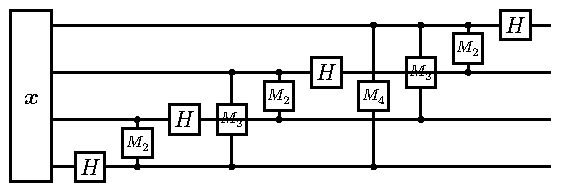
\includegraphics[width=0.9\columnwidth]{fft_tensor_network.pdf}
\caption{Complete tensor network decomposition of the 4-qubit FFT. The input tensor $\mathbf{x}$ is decomposed through Hadamard gates $H$ and controlled-phase gates $M_k$, yielding the butterfly structure of the Cooley--Tukey algorithm.}
\label{fig:fft_tn}
\end{figure}

% ============================================================================
% CIRCUIT TOPOLOGIES
% ============================================================================
\section{Parametric Circuit Topologies}
\label{sec:circuits}

We now describe four circuit topologies, each defining a parametric unitary transform $\TT(\boldsymbol{\theta}): \CC^{2^m \times 2^n} \to \CC^{2^m \times 2^n}$.
All topologies share the same gate parameterization: Hadamard-like gates $H \in U(2)$ and controlled-phase gates $M = \diag(1, 1, 1, e^{i\phi}) \in U(1)^4$ with learnable parameters.
Setting all parameters to their QFT values recovers the classical DFT.

\subsection{QFT basis}
\label{sec:qft}

The QFT basis directly parameterizes the tensor network of~\cref{sec:gate_decomposition}.
Each gate becomes a learnable parameter: the $m + n$ Hadamard gates live on $U(2)$ and the $m(m-1)/2 + n(n-1)/2$ controlled-phase gates live on $U(1)^4$.
The row and column circuits operate independently, yielding the separable transform $\TT = F_m(\boldsymbol{\theta}_{\text{row}}) \otimes F_n(\boldsymbol{\theta}_{\text{col}})$.

\textbf{Parameter count.}
For an image of size $2^m \times 2^n$: $(m + n)$ unitary gates on $U(2)$ (4 real parameters each) plus $m(m-1)/2 + n(n-1)/2$ phase gates on $U(1)^4$ (1 real parameter each), giving $4(m+n) + m(m-1)/2 + n(n-1)/2$ total real parameters.

\subsection{Entangled QFT basis}
\label{sec:entangled_qft}

The separable QFT processes row and column dimensions independently, ignoring spatial correlations between them.
Natural images exhibit strong cross-dimensional correlations (e.g., diagonal edges, radial textures).
We propose an \emph{Entangled QFT} that introduces controlled-phase gates coupling corresponding row and column qubits.

For a square image with $n$ qubits per dimension, we add $n$ entanglement gates $E_k = \diag(1, 1, 1, e^{i\phi_k})$ acting on qubit pairs $(x_{n-k}, y_{n-k})$ for $k = 1, \ldots, n$.
Each gate multiplies a learnable phase $e^{i\phi_k}$ when both the row qubit $x_{n-k}$ and column qubit $y_{n-k}$ are in state $\ket{1}$.

The total transformation is:
\begin{equation}
  \TT_{\text{entangled}} = U_{\text{entangle}} \cdot (F_n \otimes F_n),
  \quad
  U_{\text{entangle}} = \prod_{k=1}^n E_k.
  \label{eq:entangled_qft}
\end{equation}

This extension has several properties:
\begin{enumerate}
  \item Computational complexity remains $O(N \log N)$ per dimension.
  \item Only $n$ additional real parameters are introduced ($O(\log N)$ overhead).
  \item Setting $\phi_k = 0$ for all $k$ recovers the separable QFT.
\end{enumerate}

\begin{figure*}[t]
\centering
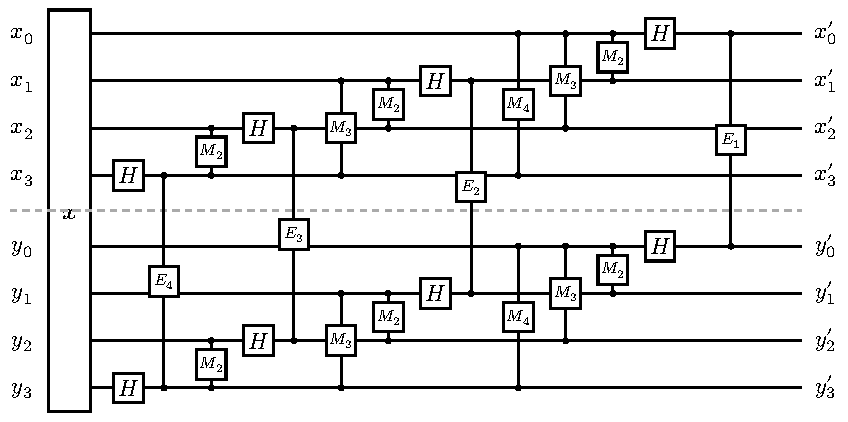
\includegraphics[width=0.85\textwidth]{entangled_qft_circuit.pdf}
\caption{Entangled QFT circuit for $n=4$ qubits per dimension. Row qubits $x_k$ and column qubits $y_k$ each pass through independent QFT circuits (Hadamard gates $H$ and controlled-phase gates $M_j$). Entanglement gates $E_k$ couple corresponding row--column pairs, introducing cross-dimensional correlations.}
\label{fig:entangled_qft}
\end{figure*}

\subsection{TEBD basis}
\label{sec:tebd}

Time-Evolving Block Decimation (TEBD)~\cite{vidal2004tebd} uses a \emph{ring topology} of nearest-neighbor controlled-phase gates preceded by Hadamard gates on each qubit.
For $n$ row qubits and $n$ column qubits, each register forms an independent ring: qubit $q_i$ is connected to $q_{i+1}$ (with wrap-around $q_n \to q_1$).

Each gate is a controlled-phase gate $T_k = \diag(1, 1, 1, e^{i\phi_k})$ with a single learnable phase.
The row ring has $n$ gates and the column ring has $n$ gates, giving $2n$ total learnable phases.
The TEBD circuit evaluates in $O(n)$ gate operations per dimension, making it the computationally cheapest basis at inference time.

The parameter manifold is:
\begin{equation}
  \MM_{\text{TEBD}} = \prod_{k=1}^{2n} U(1)^4.
\end{equation}

\begin{figure}[t]
\centering
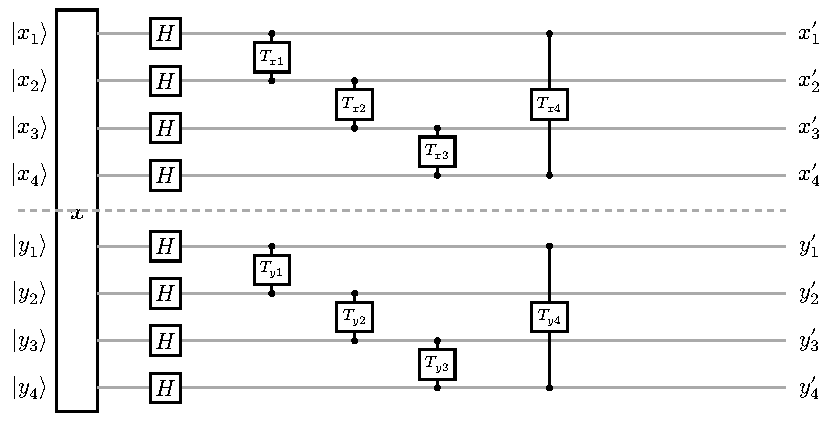
\includegraphics[width=0.9\columnwidth]{tebd_circuit.pdf}
\caption{TEBD circuit for $n=4$ row and column qubits with ring topology. Hadamard gates $H$ precede nearest-neighbor controlled-phase gates $T_{xk}$ (row ring) and $T_{yk}$ (column ring). Wrap-around gates close each ring.}
\label{fig:tebd}
\end{figure}

\subsection{MERA-inspired basis}
\label{sec:mera}

The Multi-scale Entanglement Renormalization Ansatz (MERA)~\cite{vidal2007mera} uses hierarchical connectivity with \emph{disentanglers} and \emph{isometries} at increasing spatial scales.
Our MERA-inspired basis borrows MERA's connectivity pattern while using controlled-phase gates (rather than full $U(4)$ unitaries) for consistency with the other bases and to preserve invertibility.

For $n = 2^k$ qubits, the circuit has $k = \log_2 n$ layers.
Layer $l$ has stride $s = 2^{l-1}$ and contains $n/(2s)$ pairs of disentangler and isometry gates.
Both gate types use the same parameterization: $\diag(1, 1, 1, e^{i\phi})$ with one learnable phase per gate.

The total gate count per dimension is $2(n-1)$, and the circuit depth is $O(\log n)$.
The hierarchical connectivity captures multi-scale features: layer~1 acts on nearest neighbors (fine scale), while deeper layers connect distant qubits (coarse scale).

\begin{figure*}[t]
\centering
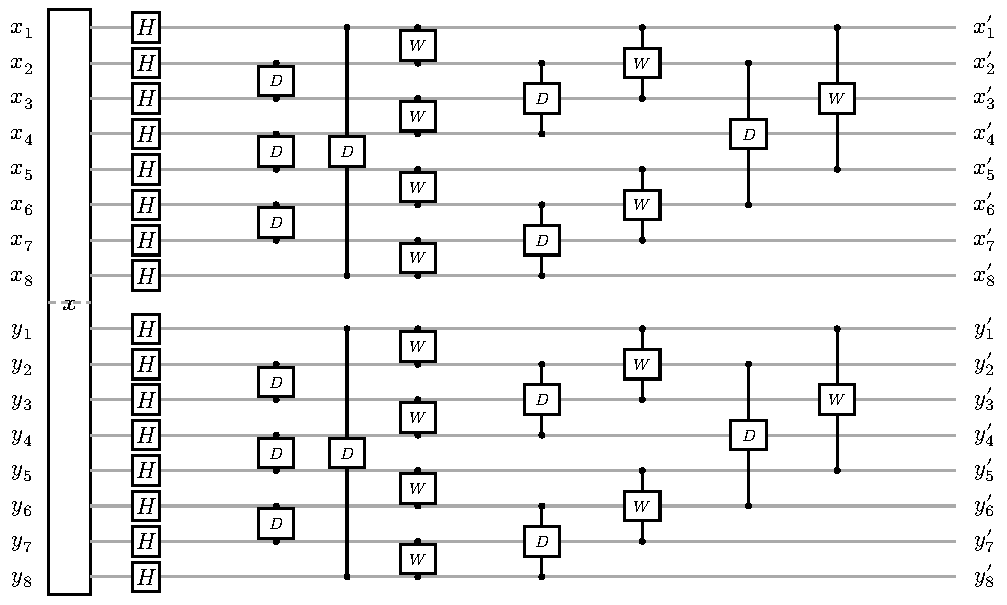
\includegraphics[width=0.85\textwidth]{mera_circuit.pdf}
\caption{MERA-inspired circuit for $n=8$ row and column qubits. Disentanglers $D$ and isometries $W$ follow hierarchical connectivity: layer~1 (stride~1) connects nearest neighbors, layer~2 (stride~2) at distance~2, layer~3 (stride~4) connects distant qubits.}
\label{fig:mera}
\end{figure*}

\subsection{Summary of circuit properties}

\begin{table}[h]
\centering
\caption{Comparison of the four circuit topologies for an image of size $2^n \times 2^n$ ($n$ qubits per dimension).}
\label{tab:circuits}
\begin{tabular}{@{}lcccc@{}}
\toprule
\textbf{Property} & \textbf{QFT} & \textbf{Ent.\ QFT} & \textbf{TEBD} & \textbf{MERA} \\
\midrule
Connectivity & all-to-all & all-to-all + XY & ring & hierarchical \\
Phase params & $n(n-1)$ & $n(n-1) + n$ & $2n$ & $4(n-1)$ \\
$U(2)$ gates & $2n$ & $2n$ & $2n$ & $2n$ \\
Circuit depth & $O(n^2)$ & $O(n^2)$ & $O(n)$ & $O(n \log n)$ \\
XY coupling & No & Yes & No & No \\
\bottomrule
\end{tabular}
\end{table}

% ============================================================================
% TRAINING
% ============================================================================
\section{Training Objective and Optimization}
\label{sec:training}

\subsection{Loss functions}

We consider three loss functions with different trade-offs between sparsity promotion and reconstruction quality.

\paragraph{$L_1$ norm loss.}
$\LL_{L_1}(\boldsymbol{\theta}) = \sum_{i,j} |\TT(\boldsymbol{\theta})(\mathbf{x})_{i,j}|$.
The $\ell_1$ norm is the tightest convex relaxation of the $\ell_0$ pseudo-norm, promoting sparse representations.

\paragraph{$L_2$ norm loss.}
$\LL_{L_2}(\boldsymbol{\theta}) = \sum_{i,j} |\TT(\boldsymbol{\theta})(\mathbf{x})_{i,j}|^2$.
Encourages energy concentration with smoother gradients than $L_1$.

\paragraph{MSE reconstruction loss.}
\begin{equation}
  \LL_{\text{MSE}}(\boldsymbol{\theta}) = \|\mathbf{x} - \TT(\boldsymbol{\theta})^{-1}(\topk(\TT(\boldsymbol{\theta})(\mathbf{x}), k))\|_F^2,
  \label{eq:mse_loss}
\end{equation}
where $\topk(\cdot, k)$ retains the $k$ coefficients with the highest frequency-weighted scores and zeros out the rest.
This loss directly optimizes reconstruction quality after truncation and is used in all experiments.

\subsection{Frequency-weighted truncation}
\label{sec:truncation}

The top-$k$ selection uses a frequency-weighted score rather than raw magnitude:
\begin{equation}
  s_{i,j} = |y_{i,j}| \cdot (1 + w_{i,j}),
  \quad
  w_{i,j} = 1 - \frac{d_{i,j}}{2\, d_{\max}},
\end{equation}
where $d_{i,j} = \sqrt{(i - c_i)^2 + (j - c_j)^2}$ is the distance from frequency bin $(i,j)$ to the DC component and $d_{\max}$ is the maximum such distance.
Low-frequency coefficients receive up to a $2\times$ boost in their retention score, consistent with the human visual system's greater sensitivity to low-frequency content.

\subsection{Straight-through gradient for top-$k$}
\label{sec:topk_grad}

The top-$k$ truncation is non-differentiable: the set of retained indices changes discontinuously.
We define a custom chain rule that passes gradients through retained coefficients and zeros out the rest---the \emph{straight-through estimator} applied to truncation:
\begin{equation}
  \frac{\partial \topk(\mathbf{y}, k)}{\partial y_{i,j}} =
  \begin{cases}
    1 & \text{if } (i,j) \in \mathcal{S}, \\
    0 & \text{otherwise},
  \end{cases}
\end{equation}
where $\mathcal{S}$ is the set of retained indices.
This is justified because (i) the true Jacobian has delta-function contributions at the boundaries that are unusable for gradient-based optimization, (ii) the mask is locally stable during training, and (iii) the gradient correctly conveys ``adjust the retained coefficients to better approximate the signal.''

\subsection{Riemannian optimization}
\label{sec:riemannian}

The circuit parameters live on two manifolds:

\begin{definition}[Unitary manifold $U(2)$]
The group of $2 \times 2$ unitary matrices with tangent space $T_U U(2) = \{US : S^\dagger = -S\}$.
\end{definition}

\begin{definition}[Phase manifold $U(1)^4$]
The product of four unit circles with tangent space $T_{\mathbf{z}} U(1)^4 = \{i\boldsymbol{\theta} \circ \mathbf{z} : \boldsymbol{\theta} \in \RR^4\}$.
\end{definition}

\paragraph{Riemannian gradient.}
Given the Euclidean gradient $\nabla_E f$ from automatic differentiation:
\begin{align}
  \text{For } U(2): & \quad \grad f(U) = U \cdot \skew(U^\dagger \nabla_E f), \label{eq:grad_u2} \\
  \text{For } U(1)^4: & \quad \grad f(\mathbf{z}) = i \cdot \operatorname{Im}(\bar{\mathbf{z}} \circ \nabla_E f) \circ \mathbf{z}, \label{eq:grad_u1}
\end{align}
where $\skew(A) = (A - A^\dagger)/2$ extracts the skew-Hermitian part.

\paragraph{Retraction.}
For $U(2)$, we use the Cayley retraction:
\begin{equation}
  R_U(\alpha \xi) = \left(I - \frac{\alpha}{2} W\right)^{-1} \left(I + \frac{\alpha}{2} W\right) U,
  \label{eq:cayley}
\end{equation}
where $W = \xi U^\dagger$ projected to $\mathfrak{u}(2)$ via $W \leftarrow (W - W^\dagger)/2$.
The Cayley map preserves unitarity exactly for any step size $\alpha$.
For $U(1)^4$, we use normalization: $R_{\mathbf{z}}(\alpha \xi) = (\mathbf{z} + \alpha \xi) / |\mathbf{z} + \alpha \xi|$ elementwise.

\paragraph{Riemannian gradient descent with Armijo line search.}
The update rule is $x_{t+1} = R_{x_t}(-\eta \cdot \grad f(x_t))$, where $\eta$ is determined by Armijo backtracking: starting from $\alpha_0$, contract $\alpha \leftarrow \tau \alpha$ (with $\tau = 0.5$) until the sufficient decrease condition is satisfied:
\begin{equation}
  \LL(R_{x_t}(-\alpha \cdot \grad f(x_t))) \leq \LL(x_t) - c \cdot \alpha \cdot \|\grad f(x_t)\|^2,
\end{equation}
with $c = 10^{-4}$.

\paragraph{Riemannian Adam.}
We also implement Riemannian Adam~\cite{becigneul2019riemannian}, which maintains exponentially weighted first and second moment estimates of the Riemannian gradient with parallel transport of momentum between iterates.
The bias-corrected update direction is $d_t = \hat{m}_t / (\sqrt{\hat{v}_t} + \epsilon)$, with $\beta_1 = 0.9$, $\beta_2 = 0.999$, $\epsilon = 10^{-8}$.
Momentum is transported between tangent spaces via projection:
\begin{equation}
  \Gamma_{x_t \to x_{t+1}}(m_t) = \proj_{T_{x_{t+1}} \MM}(m_t).
\end{equation}

\subsection{Batched einsum evaluation}

The forward transform is implemented as an Einstein summation (einsum) contraction of the image tensor with the gate tensors.
The contraction order is pre-optimized using a tree search algorithm (TreeSA) that minimizes the total operation count.

For batched training, a batch index $\beta$ is appended to the image input/output indices:
\begin{equation}
  Y_{q'_1, \ldots, q'_{m+n}, \beta} = \sum_{q_1, \ldots, q_{m+n}} \left(\prod_j G^j_{\cdots}\right) X_{q_1, \ldots, q_{m+n}, \beta}.
\end{equation}
The gate tensors are shared across the batch, reducing GPU kernel launch overhead from $O(B)$ to $O(1)$.

% ============================================================================
% EXPERIMENTS
% ============================================================================
\section{Experiments}
\label{sec:experiments}

\subsection{Setup}

\paragraph{Datasets.}
We evaluate on three datasets of increasing scale:
\begin{itemize}
  \item \textbf{Quick Draw}~\cite{quickdraw}: Hand-drawn sketches ($28 \times 28$, zero-padded to $32 \times 32$, i.e., $m = n = 5$ qubits). Five categories (cat, dog, airplane, apple, bicycle), 1000+ images per category.
  \item \textbf{DIV2K}~\cite{div2k}: High-resolution natural photographs, preprocessed to $256 \times 256$ ($m = n = 8$ qubits). 800 training + 100 validation images.
  \item \textbf{CLIC}: Professional photographs from the CLIC challenge, preprocessed to $512 \times 512$ ($m = n = 9$ qubits). This dataset tests scalability to higher resolutions with rich texture and detail.
\end{itemize}

\paragraph{Training configuration.}
All bases are trained using RiemannianGD with Armijo line search ($\alpha_0 = 0.01$, $c = 10^{-4}$, $\tau = 0.5$, max 10 backtracking steps).
The primary loss function is $\LL_{\text{MSE}}$ (\cref{eq:mse_loss}) with $k = 10\%$ of total coefficients.
We additionally train all bases with the $L_1$ norm loss to evaluate the effect of sparsity-promoting objectives.
We use a 20\% validation split, early stopping with patience 2 epochs, and random seed 42 for reproducibility.

\paragraph{Metrics.}
We report PSNR (peak signal-to-noise ratio, $10 \log_{10}(1/\text{MSE})$, higher is better) and SSIM (structural similarity index, higher is better) at compression ratios $k/N \in \{5\%, 10\%, 15\%, 20\%\}$.
All metrics are averaged over the full evaluation set.

\paragraph{Baselines.}
We compare against the classical FFT (the untrained fixed-parameter DFT) and the DCT (Discrete Cosine Transform), which serve as natural baselines since the FFT is the initialization point for all learned bases and the DCT is the standard transform used in JPEG compression.

\subsection{MSE Loss Results}

\begin{table}[h]
\centering
\caption{Compression quality on Quick Draw ($32 \times 32$, MSE loss). PSNR (dB) / SSIM at four compression ratios. Best learned result in \textbf{bold}.}
\label{tab:quickdraw_mse}
\resizebox{\columnwidth}{!}{\input{tables/quickdraw_mse}}
\end{table}

\begin{table}[h]
\centering
\caption{Compression quality on DIV2K ($256 \times 256$, MSE loss). PSNR (dB) / SSIM.}
\label{tab:div2k_mse}
\resizebox{\columnwidth}{!}{\input{tables/div2k_mse}}
\end{table}

\begin{table}[h]
\centering
\caption{Compression quality on CLIC ($512 \times 512$, MSE loss). PSNR (dB) / SSIM.}
\label{tab:clic_mse}
\resizebox{\columnwidth}{!}{\input{tables/clic_mse}}
\end{table}

\begin{figure*}[t]
\centering
\includegraphics[width=0.32\textwidth]{mse/quickdraw_reconstruction_grid.png}
\includegraphics[width=0.32\textwidth]{mse/div2k_reconstruction_grid.png}
\includegraphics[width=0.32\textwidth]{mse/clic_reconstruction_grid.png}
\caption{Reconstruction quality comparison across datasets (MSE loss). Each grid shows the original image and reconstructions at 5\%, 10\%, 15\%, and 20\% coefficient retention for each basis type.}
\label{fig:recon_mse}
\end{figure*}

\begin{figure}[t]
\centering
\includegraphics[width=0.48\columnwidth]{mse/cross_dataset_psnr.png}
\includegraphics[width=0.48\columnwidth]{mse/cross_dataset_ssim.png}
\caption{Cross-dataset comparison of PSNR and SSIM at 10\% coefficient retention (MSE loss).}
\label{fig:cross_mse}
\end{figure}

Across all three datasets (\cref{tab:quickdraw_mse,tab:div2k_mse,tab:clic_mse}), the Entangled QFT achieves the best or tied-best performance among learned bases at every compression ratio.
On Quick Draw, the Entangled QFT improves over the classical FFT by up to $+0.20$~dB PSNR and $+0.015$ SSIM at 20\% compression.
The separable QFT shows modest gains at aggressive compression (5\%) but converges to FFT performance at higher ratios, suggesting that the learned parameters remain close to the DFT values.
TEBD consistently underperforms the fixed FFT baseline, indicating that the ring topology's nearest-neighbor connectivity is insufficient for the frequency structure of images.

On DIV2K and CLIC, the QFT-family bases improve over the FFT baseline, with the Entangled QFT and separable QFT performing comparably.
The gain from entanglement is smaller on high-resolution images, likely because the 8- and 9-qubit QFT structures already provide sufficient all-to-all connectivity within each dimension.
TEBD's deficit grows with image complexity, consistent with the expectation that the ring topology's locality becomes more limiting as resolution increases.

\subsection{L1 Norm Results}

To compare the effect of loss function choice, we also train all bases using the L1 norm loss, which promotes sparsity via compressed sensing theory.

\begin{table}[h]
\centering
\caption{Compression quality on Quick Draw ($32 \times 32$, L1 norm loss). PSNR (dB) / SSIM.}
\label{tab:quickdraw_l1}
\resizebox{\columnwidth}{!}{\input{tables/l1norm_quickdraw}}
\end{table}

\begin{figure*}[t]
\centering
\includegraphics[width=0.32\textwidth]{l1norm/quickdraw_reconstruction_grid.png}
\includegraphics[width=0.32\textwidth]{l1norm/div2k_reconstruction_grid.png}
\includegraphics[width=0.32\textwidth]{l1norm/clic_reconstruction_grid.png}
\caption{Reconstruction quality comparison (L1 norm loss).}
\label{fig:recon_l1}
\end{figure*}

The L1 norm loss promotes coefficient sparsity more aggressively than the MSE reconstruction loss.
However, because the L1 objective does not directly optimize reconstruction quality after truncation, the MSE-trained bases generally achieve higher PSNR and SSIM at the same compression ratio.
The relative ranking of circuit topologies is preserved under both loss functions: the Entangled QFT remains the strongest learned basis, and TEBD remains the weakest, confirming that the topology effect is robust to the choice of training objective.

\subsection{Topology Comparison (8-qubit, $256 \times 256$)}

To compare all four topologies including MERA (which requires power-of-two qubit counts), we evaluate on DIV2K at $256 \times 256$ resolution ($m = n = 8$ qubits).

\begin{table}[h]
\centering
\caption{Topology comparison on DIV2K ($256 \times 256$, 8 qubits). All four circuit topologies including MERA.}
\label{tab:topology}
\resizebox{\columnwidth}{!}{\input{tables/div2k_8q}}
\end{table}

\begin{figure}[t]
\centering
\includegraphics[width=0.9\columnwidth]{topology/div2k_8q_reconstruction_grid.png}
\caption{Reconstruction grid for all four topologies on DIV2K ($256 \times 256$, 8 qubits).}
\label{fig:recon_topology}
\end{figure}

\begin{figure}[t]
\centering
\includegraphics[width=0.9\columnwidth]{topology/div2k_8q_training_curves.png}
\caption{Training convergence for all four topologies on DIV2K (8 qubits).}
\label{fig:training_topology}
\end{figure}

The MERA-inspired basis, with its hierarchical multi-scale connectivity and $O(\log n)$ circuit depth, captures features at multiple spatial scales.
Its performance falls between the QFT-family bases and TEBD, consistent with the observation that hierarchical connectivity is more expressive than ring connectivity but less so than the all-to-all connectivity of the QFT variants.

\subsection{Training Dynamics}

\begin{table}[h]
\centering
\caption{Training time (seconds) across datasets (MSE loss).}
\label{tab:timing}
\resizebox{\columnwidth}{!}{\input{tables/timing}}
\end{table}

\begin{figure}[t]
\centering
\includegraphics[width=0.48\columnwidth]{mse/quickdraw_training_curves.png}
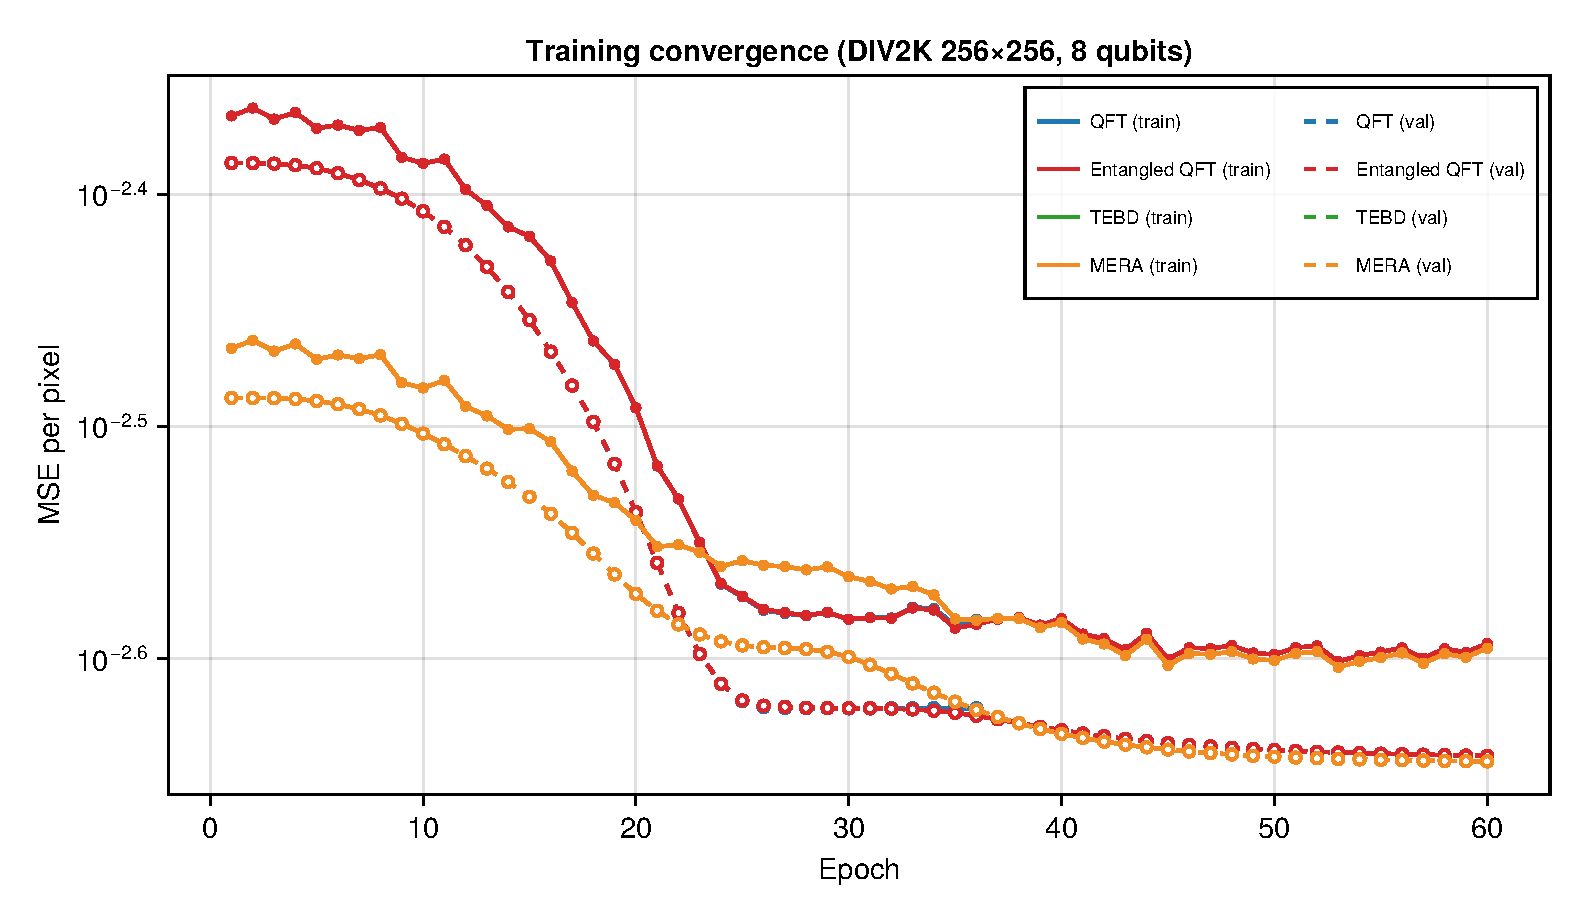
\includegraphics[width=0.48\columnwidth]{mse/div2k_training_curves.png}
\caption{Training convergence curves (MSE loss). Validation loss vs.\ epoch on log scale.}
\label{fig:training_curves}
\end{figure}

\begin{figure}[t]
\centering
\includegraphics[width=0.48\columnwidth]{mse/quickdraw_step_losses.png}
\includegraphics[width=0.48\columnwidth]{mse/div2k_step_losses.png}
\caption{Per-step training loss (MSE loss).}
\label{fig:step_losses}
\end{figure}

The Entangled QFT converges faster than the separable QFT despite having more parameters.
We attribute this to the cross-dimensional gradient pathways created by the entanglement gates, which provide additional directions for the optimizer to explore.
TEBD converges to a higher training loss than the QFT variants.
Notably, TEBD's validation loss is lower than its training loss, suggesting that the ring topology acts as an implicit regularizer at the cost of underfitting.

\subsection{Effect of circuit topology}

The key experimental finding is that \textbf{circuit connectivity topology determines compression quality more than parameter count or circuit depth}:

\begin{enumerate}
  \item The Entangled QFT adds only $n$ phase parameters over the QFT ($+8$ parameters for DIV2K) yet consistently achieves the best or tied-best performance.
  \item TEBD has $2n$ phase parameters---comparable to the Entangled QFT---but performs worst due to its local ring connectivity.
  \item The MERA-inspired basis, with hierarchical connectivity, performs between QFT and TEBD, demonstrating that multi-scale structure is beneficial but insufficient without cross-dimensional coupling.
  \item The QFT's all-to-all connectivity within each dimension closely matches the DFT's frequency structure, explaining why learned QFT bases converge near the DFT solution.
  \item Cross-dimensional coupling (Entangled QFT) captures correlations that no amount of intra-dimensional parameters can express in a separable architecture.
\end{enumerate}

% ============================================================================
% DISCUSSION
% ============================================================================
\section{Discussion}
\label{sec:discussion}

The learned bases improve upon the classical FFT but do not dramatically exceed it.
This is consistent with the DFT being near-optimal within the separable transform family for generic images~\cite{donoho2006compressed}: the separable QFT's learned parameters converge close to DFT values, confirming that the FFT occupies a strong local minimum on the parameter manifold.
The Entangled QFT improves upon this by expanding the search space with cross-dimensional connections that the separable manifold cannot reach.
Results on CLIC ($512 \times 512$) confirm that these findings scale to higher resolutions.

The comparison between the Entangled QFT and TEBD is instructive for quantum circuit design.
The Entangled QFT's $n$ cross-dimensional phases outperform TEBD's $2n$ ring-topology phases because they connect degrees of freedom that are relevant to the 2D structure of images.
The entanglement gates enable the basis to represent frequency components that mix row and column information, which no separable architecture can express regardless of parameter count.
The MERA-inspired basis, with its hierarchical multi-scale connectivity, performs between the QFT variants and TEBD (\cref{tab:topology}), confirming that multi-scale structure is beneficial but insufficient without cross-dimensional coupling.
This observation suggests that for variational quantum circuits, the connectivity pattern should be guided by the structure of the target problem rather than chosen for computational convenience.

The comparison of MSE and L1 training objectives reveals that the relative ranking of circuit topologies is robust to the choice of loss function (\cref{tab:quickdraw_l1}).
While the L1 norm promotes sparsity more aggressively, the MSE reconstruction loss yields better compression metrics because it directly optimizes the end-to-end reconstruction pipeline including truncation.

While our circuits are evaluated classically as tensor networks, the parametric QFT structure maps directly to quantum hardware: implementing the Entangled QFT requires only $n$ additional CPHASE gates beyond the standard QFT circuit.
The tensor network contraction framework used in this work shares the same computational structure as quantum circuit simulation~\cite{luo2020yao, markov2008simulating}, and can exploit the same software and hardware advances, including GPU acceleration and optimized contraction orders.

The inclusion of the DCT as a baseline provides context for the learned bases: the DCT's real-valued cosine basis is well-suited for natural images, and comparisons against it quantify the practical advantage of learned unitary transforms.
Ablation studies isolating the contribution of Riemannian vs.\ projected Euclidean optimization, and comparison with wavelets and learned dictionaries, are natural next steps.
A Julia implementation of the framework is available as an open-source library.
% TODO: Add URL/DOI when available.

% ============================================================================
% CONCLUSION
% ============================================================================
\section{Conclusion}

We have presented a framework for learning parametric quantum circuit bases for image compression, optimized on Riemannian manifolds of unitary and phase gates.
By systematically comparing four circuit topologies, we find that circuit connectivity topology is a more important design variable than parameter count or circuit depth: the Entangled QFT, with $O(\log N)$ additional cross-dimensional gates, consistently outperforms topologies with comparable or greater parameter counts, while TEBD's local ring connectivity degrades below the fixed FFT baseline.

The framework unifies tensor network contraction, Riemannian optimization, and differentiable programming into a single pipeline.
New circuit topologies can be defined by specifying a connectivity pattern; the manifold optimization, batched einsum evaluation, and differentiable truncation machinery apply unchanged.
The approach adds another example along the fruitful line of research combining tensor networks, automatic differentiation, and quantum circuit structures for computational applications.

% ============================================================================
% ACKNOWLEDGMENTS
% ============================================================================
\begin{acknowledgments}
% TODO: Add acknowledgments.
\end{acknowledgments}

% ============================================================================
% REFERENCES
% ============================================================================
\bibliography{references}
\bibliographystyle{unsrt}

% ============================================================================
% APPENDICES
% ============================================================================
\appendix

\section{Riemannian optimization details}
\label{app:riemannian}

\subsection{Cayley retraction derivation}

For a unitary matrix $U \in U(2)$ and tangent vector $\xi = US$ where $S^\dagger = -S$, the Cayley retraction maps:
\begin{align}
  W &= \xi U^\dagger = USU^\dagger, \\
  W &\leftarrow \frac{W - W^\dagger}{2} \quad \text{(project to } \mathfrak{u}(2)\text{)}, \\
  R_U(\alpha \xi) &= \left(I - \frac{\alpha}{2}W\right)^{-1}\left(I + \frac{\alpha}{2}W\right)U.
\end{align}

Since $W$ is skew-Hermitian, $(I - \frac{\alpha}{2}W)^{-1}(I + \frac{\alpha}{2}W)$ is unitary for any $\alpha \in \RR$, as can be verified by checking that the product with its adjoint equals the identity.

For $2 \times 2$ matrices, the inverse admits a closed form via the adjugate:
\begin{equation}
  (I - \frac{\alpha}{2}W)^{-1} = \frac{1}{\det(I - \frac{\alpha}{2}W)} \operatorname{adj}(I - \frac{\alpha}{2}W).
\end{equation}

\subsection{Parallel transport for Riemannian Adam}

For $U(2)$, the projection-based transport from $U_t$ to $U_{t+1}$ is:
\begin{equation}
  \Gamma_{U_t \to U_{t+1}}(m_t) = U_{t+1} \cdot \skew(U_{t+1}^\dagger m_t).
\end{equation}

For $U(1)^4$, the transport is the tangent projection at the new point:
\begin{equation}
  \Gamma_{\mathbf{z}_t \to \mathbf{z}_{t+1}}(m_t) = i \cdot \operatorname{Im}(\bar{\mathbf{z}}_{t+1} \circ m_t) \circ \mathbf{z}_{t+1}.
\end{equation}

Both are exact to first order in the step size.

\section{Detailed benchmark configurations}
\label{app:benchmark}

\begin{table}[h]
\centering
\caption{Hyperparameters used in the benchmark experiments.}
\begin{tabular}{@{}ll@{}}
\toprule
\textbf{Parameter} & \textbf{Value} \\
\midrule
Optimizer & RiemannianGD \\
Initial learning rate $\alpha_0$ & 0.01 \\
Armijo constant $c$ & $10^{-4}$ \\
Backtracking factor $\tau$ & 0.5 \\
Max backtracking steps & 10 \\
Loss functions & MSE ($k = 10\%$), L1 norm \\
Validation split & 20\% \\
Early stopping patience & 2 epochs \\
Random seed & 42 \\
\midrule
\multicolumn{2}{@{}l}{\textbf{Quick Draw} ($32 \times 32$, $m = n = 5$ qubits)} \\
Epochs & 5 \\
Training images & 20 \\
\midrule
\multicolumn{2}{@{}l}{\textbf{DIV2K} ($256 \times 256$, $m = n = 8$ qubits)} \\
Epochs & 5 \\
Training images & 20 \\
\midrule
\multicolumn{2}{@{}l}{\textbf{CLIC} ($512 \times 512$, $m = n = 9$ qubits)} \\
Epochs & 5 \\
Training images & 20 \\
\bottomrule
\end{tabular}
\end{table}

\end{document}
